\documentclass[margin=5mm]{standalone}
\usepackage[dvipsnames]{xcolor}
\usepackage{pgfplots}
\usepackage{tikz}
\usepackage[tikz]{ocgx2}

\pgfplotsset{compat=1.18}
\begin{document}

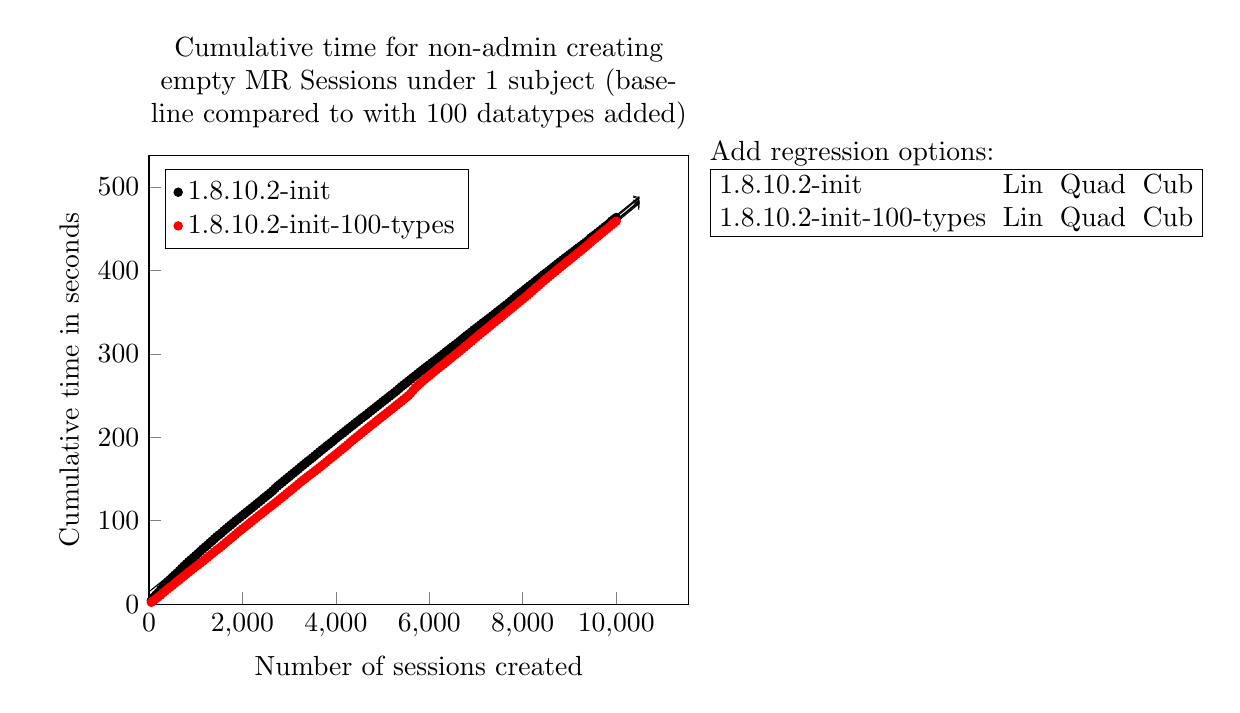
\begin{tikzpicture}
    \begin{axis}[
        align = center,
        legend pos = north west,
        legend cell align = left,
        xlabel = Number of sessions created,
        ylabel = Cumulative time in seconds,
        xtick pos = left,
        ytick pos = left,
        scaled ticks = false,
        xmin = 0,
        ymin = 0,
        title = {Cumulative time for non-admin creating empty MR Sessions under 1 subject  (baseline compared to with 100 datatypes added)},
        title style = {text width = 0.8\textwidth},
        legend entries={\switchocg{1.8.10.2-init}{1.8.10.2-init},\switchocg{1.8.10.2-init-100-types}{1.8.10.2-init-100-types}}]
        \begin{scope}[ocg = {ref = 1.8.10.2-init-Lin, status = invisible}]
            \plot[domain=0:10500,->,forget plot] (\x,{14.8587102512562072575974525534547865390777587890625 + 0.045095791989799745291822574699835968203842639923095703125*(\x)^1});
        \end{scope}
        \begin{scope}[ocg = {ref = 1.8.10.2-init-Quad, status = invisible}]
            \plot[domain=0:10500,->,forget plot] (\x,{9.5256347944265851168665903969667851924896240234375 + 0.0482639556275203107649218736696639098227024078369140625*(\x)^1 + -0.00000031524016295727027632233283906126874995834441506303846836090087890625*(\x)^2});
        \end{scope}
        \begin{scope}[ocg = {ref = 1.8.10.2-init-Cub, status = invisible}]
            \plot[domain=0:10500,->,forget plot] (\x,{6.05828095960488877125271756085567176342010498046875 + 0.052353176997400475978228229223532252945005893707275390625*(\x)^1 + -0.00000132992694093758422564720104996904836980320396833121776580810546875*(\x)^2 + 0.0000000000673092390036692228434191737879263746358038389416833524592220783233642578125*(\x)^3});
        \end{scope}
        \begin{scope}[ocg = {ref = 1.8.10.2-init, status = visible}]
            \addplot[
                only marks,
                color = black,
                mark = *,
                mark size = 1.5 pt
            ]coordinates {(50,4.426)(100,7.871)(150,11.067)(200,14.13)(250,17.602)(300,20.766)(350,23.723)(400,26.75)(450,29.417)(500,32.204)(550,34.725)(600,37.305)(650,40.1)(700,42.838)(750,45.707)(800,48.265)(850,50.938)(900,53.346)(950,55.861)(1000,58.258)(1050,60.793)(1100,63.432)(1150,66.064)(1200,68.41)(1250,70.754)(1300,73.357)(1350,75.769)(1400,78.31)(1450,80.77)(1500,83.041)(1550,85.238)(1600,87.857)(1650,90.184)(1700,92.579)(1750,94.818)(1800,97.176)(1850,99.639)(1900,101.786)(1950,104.061)(2000,106.309)(2050,108.487)(2100,110.787)(2150,113.086)(2200,115.234)(2250,117.545)(2300,119.8)(2350,122.149)(2400,124.368)(2450,126.799)(2500,128.997)(2550,131.237)(2600,133.538)(2650,135.863)(2700,138.771)(2750,141.369)(2800,143.606)(2850,145.876)(2900,148.218)(2950,150.483)(3000,152.782)(3050,155.074)(3100,157.348)(3150,159.694)(3200,161.922)(3250,164.373)(3300,166.619)(3350,168.908)(3400,171.193)(3450,173.346)(3500,175.522)(3550,177.872)(3600,180.232)(3650,182.561)(3700,184.807)(3750,186.99)(3800,189.366)(3850,191.484)(3900,193.684)(3950,195.878)(4000,198.389)(4050,200.597)(4100,202.828)(4150,204.964)(4200,207.213)(4250,209.466)(4300,211.676)(4350,213.877)(4400,216.162)(4450,218.337)(4500,220.477)(4550,222.738)(4600,224.802)(4650,226.904)(4700,229.207)(4750,231.434)(4800,233.599)(4850,235.826)(4900,238.033)(4950,240.244)(5000,242.516)(5050,244.725)(5100,246.856)(5150,249.091)(5200,251.222)(5250,253.449)(5300,255.62)(5350,258.129)(5400,260.566)(5450,262.705)(5500,264.924)(5550,267.137)(5600,269.366)(5650,271.648)(5700,273.777)(5750,275.991)(5800,278.308)(5850,280.431)(5900,282.631)(5950,284.732)(6000,286.796)(6050,288.992)(6100,291.168)(6150,293.281)(6200,295.483)(6250,297.536)(6300,299.702)(6350,302.046)(6400,304.243)(6450,306.494)(6500,308.55)(6550,310.717)(6600,312.844)(6650,314.978)(6700,317.38)(6750,319.709)(6800,321.866)(6850,323.983)(6900,326.166)(6950,328.522)(7000,330.682)(7050,332.766)(7100,334.869)(7150,337.089)(7200,339.198)(7250,341.355)(7300,343.511)(7350,345.656)(7400,347.716)(7450,350.07)(7500,352.198)(7550,354.409)(7600,356.625)(7650,358.775)(7700,360.978)(7750,363.31)(7800,365.689)(7850,368.306)(7900,370.496)(7950,372.702)(8000,374.897)(8050,377.254)(8100,379.497)(8150,381.561)(8200,383.744)(8250,385.929)(8300,388.34)(8350,390.439)(8400,392.805)(8450,395.035)(8500,397.126)(8550,399.182)(8600,401.462)(8650,403.624)(8700,405.884)(8750,408.133)(8800,410.261)(8850,412.367)(8900,414.592)(8950,416.69)(9000,418.867)(9050,420.93)(9100,423.098)(9150,425.253)(9200,427.298)(9250,429.443)(9300,431.508)(9350,433.702)(9400,435.857)(9450,438.622)(9500,440.789)(9550,442.859)(9600,444.933)(9650,447.116)(9700,449.527)(9750,451.768)(9800,453.885)(9850,456.237)(9900,459.015)(9950,461.226)(10000,463.291)};
        \end{scope}
        \begin{scope}[ocg = {ref = 1.8.10.2-init-100-types-Lin, status = invisible}]
            \plot[domain=0:10500,->,forget plot] (\x,{-2.518228391959621337292674070340581238269805908203125 + 0.04599409918247954198733395969611592590808868408203125*(\x)^1});
        \end{scope}
        \begin{scope}[ocg = {ref = 1.8.10.2-init-100-types-Quad, status = invisible}]
            \plot[domain=0:10500,->,forget plot] (\x,{0.055897875742585749481161627727487939409911632537841796875 + 0.044464915261072303354072943193386890925467014312744140625*(\x)^1 + 0.000000152157604120123219367175762713195741326899224077351391315460205078125*(\x)^2});
        \end{scope}
        \begin{scope}[ocg = {ref = 1.8.10.2-init-100-types-Cub, status = invisible}]
            \plot[domain=0:10500,->,forget plot] (\x,{0.809738464109789557454632813460193574428558349609375 + 0.043575873879579514469373435758825507946312427520751953125*(\x)^1 + 0.00000037276159037595113463704385968477961199596393271349370479583740234375*(\x)^2 + -0.00000000001463376359905988994454964157194564074171427847659288090653717517852783203125*(\x)^3});
        \end{scope}
        \begin{scope}[ocg = {ref = 1.8.10.2-init-100-types, status = visible}]
            \addplot[
                only marks,
                color = red,
                mark = *,
                mark size = 1.5 pt
            ]coordinates {(50,2.187)(100,4.378)(150,6.562)(200,8.737)(250,10.871)(300,13.512)(350,15.775)(400,18.106)(450,20.295)(500,22.383)(550,24.747)(600,26.98)(650,29.203)(700,31.423)(750,33.714)(800,36.034)(850,38.303)(900,40.491)(950,42.768)(1000,44.874)(1050,46.979)(1100,49.126)(1150,51.267)(1200,53.451)(1250,55.842)(1300,58.16)(1350,60.392)(1400,62.689)(1450,64.852)(1500,67.028)(1550,69.243)(1600,71.467)(1650,74.002)(1700,76.247)(1750,78.621)(1800,80.891)(1850,83.228)(1900,85.802)(1950,87.978)(2000,90.204)(2050,92.43)(2100,94.609)(2150,96.898)(2200,99.16)(2250,101.348)(2300,103.591)(2350,105.809)(2400,107.966)(2450,110.228)(2500,112.478)(2550,114.701)(2600,116.876)(2650,119.038)(2700,121.199)(2750,123.465)(2800,125.732)(2850,127.922)(2900,130.063)(2950,132.53)(3000,134.885)(3050,137.064)(3100,139.32)(3150,141.63)(3200,144.047)(3250,146.365)(3300,148.57)(3350,150.711)(3400,152.964)(3450,155.076)(3500,157.225)(3550,159.413)(3600,161.578)(3650,163.719)(3700,165.936)(3750,168.227)(3800,170.411)(3850,172.799)(3900,175.097)(3950,177.22)(4000,179.525)(4050,181.89)(4100,184.173)(4150,186.435)(4200,188.64)(4250,190.909)(4300,193.561)(4350,195.901)(4400,198.169)(4450,200.44)(4500,202.57)(4550,205.011)(4600,207.194)(4650,209.464)(4700,211.712)(4750,213.922)(4800,216.097)(4850,218.392)(4900,220.617)(4950,222.885)(5000,225.014)(5050,227.295)(5100,229.48)(5150,231.744)(5200,233.888)(5250,236.22)(5300,238.452)(5350,240.677)(5400,242.866)(5450,245.128)(5500,247.355)(5550,249.672)(5600,252.554)(5650,255.953)(5700,259.265)(5750,261.787)(5800,264.176)(5850,266.716)(5900,269.181)(5950,271.428)(6000,273.717)(6050,276.091)(6100,278.378)(6150,280.708)(6200,282.932)(6250,285.18)(6300,287.368)(6350,289.588)(6400,291.86)(6450,294.167)(6500,296.444)(6550,298.723)(6600,300.989)(6650,303.216)(6700,305.481)(6750,307.82)(6800,310.068)(6850,312.621)(6900,314.961)(6950,317.319)(7000,319.637)(7050,321.968)(7100,324.29)(7150,326.5)(7200,328.747)(7250,330.992)(7300,333.301)(7350,335.648)(7400,337.934)(7450,340.144)(7500,342.452)(7550,344.672)(7600,347.041)(7650,349.344)(7700,351.734)(7750,353.933)(7800,356.205)(7850,358.579)(7900,360.873)(7950,363.259)(8000,365.512)(8050,367.796)(8100,3.7E+2)(8150,372.643)(8200,375.092)(8250,377.668)(8300,379.906)(8350,382.231)(8400,384.89)(8450,387.351)(8500,389.674)(8550,392.111)(8600,394.363)(8650,396.603)(8700,398.856)(8750,401.178)(8800,403.555)(8850,405.764)(8900,408.023)(8950,410.264)(9000,412.54)(9050,414.788)(9100,417.043)(9150,419.351)(9200,421.629)(9250,423.932)(9300,426.212)(9350,428.427)(9400,430.788)(9450,433.43)(9500,435.817)(9550,438.108)(9600,440.377)(9650,442.668)(9700,445.118)(9750,447.347)(9800,449.615)(9850,451.852)(9900,454.256)(9950,456.476)(10000,458.816)};
        \end{scope}
    \end{axis}
    \begin{scope}
        \addtolength{\tabcolsep}{-0.3em}
        \node [below right, shape=rectangle, align=left](regressiontable) at (7,6) {
            Add regression options: \\
            \begin{tabular}{|llll|}
                \hline
                1.8.10.2-init & \switchocg{1.8.10.2-init-Lin}{Lin} & \switchocg{1.8.10.2-init-Quad}{Quad} & \switchocg{1.8.10.2-init-Cub}{Cub} \\
                1.8.10.2-init-100-types & \switchocg{1.8.10.2-init-100-types-Lin}{Lin} & \switchocg{1.8.10.2-init-100-types-Quad}{Quad} & \switchocg{1.8.10.2-init-100-types-Cub}{Cub} \\
                \hline
            \end{tabular}
        };
    \end{scope}
\end{tikzpicture}

\end{document}